\chapter{実験}
\section{シミュレーション}
シュミレーションを利用して,設計した制御系の性能を確認する.

\subsubsection{シミュレーションソフト}
シミュレーションには数値計算ソフト「Scilab」に付属しているビジュアルモデリングソフト「Xcos」を使用する.Xcosで組み立てたブロック線図を図\ref{fig:blockXcos}に示す.この際、リフトにかかる電圧の絶対値の最大は実際と同じく12[v]に制限した.

\begin{figure}[htbp]
  \begin{center}
    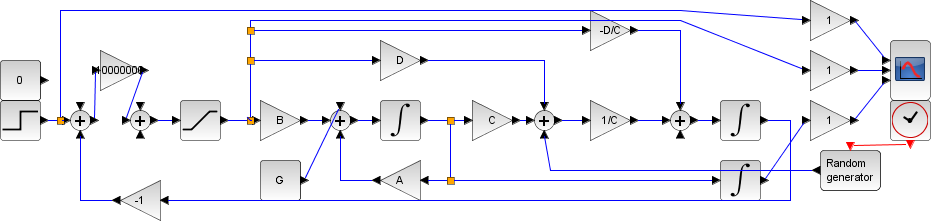
\includegraphics[width=150mm]{img/blockXcos.png}
    \end{center}
  \caption{Xcosで組み立てたブロック線図}
 \label{fig:blockXcos}
\end{figure}

\subsubsection{シミュレーション結果}
シミュレーションの結果を図\ref{fig:sim}に示す.

\begin{figure}[htbp]
 \begin{center}
    \includegraphics[width=150mm]{img/sim.bmp}
    \end{center}
  \caption{入力した目標値による電圧と位置の時間変化}
 \label{fig:sim}
\end{figure}

\subsubsection{測定誤差の影響}
実際に電流を測定した時には誤差があると考え,誤差の影響を見るため電流の値を分散が1[A]の正規分布になるようにした.その際のシミュレーション結果を図\ref{fig:sim}に示す.

\begin{figure}[htbp]
 \begin{center}
    \includegraphics[width=150mm]{img/sim2.bmp}
    \end{center}
  \caption{入力した目標値による電圧と位置の時間変化}
 \label{fig:sim}
\end{figure}

電圧のグラフが激しく振動している為,塗りつぶされて見える.これは電流の誤差の影響だと考えられるが,現在位置に影響はなかった.

\section{電流値の測定}